%\documentclass[fleqn, letterpaper]{amsart}
\documentclass[fleqn, letterpaper]{tufte-handout}
\usepackage{times}
\usepackage{amsmath}
\usepackage{graphicx}
\usepackage{booktabs}
\usepackage{multirow}
%\usepackage[left=1in]{geometry}

\newcommand{\R}{\mathcal{R}}
\newcommand{\E}{\text{E}}
\newcommand{\p}{p_{XY}}
\renewcommand{\arraystretch}{1.5}

\title{Problem Set 2 --- ENCE689E Spring 2014}
\author{David Prentiss}

\begin{document}
\maketitle


\section{1. Monte Carlo Methods}
\subsection{(h)}
\begin{figure*}[h!]
        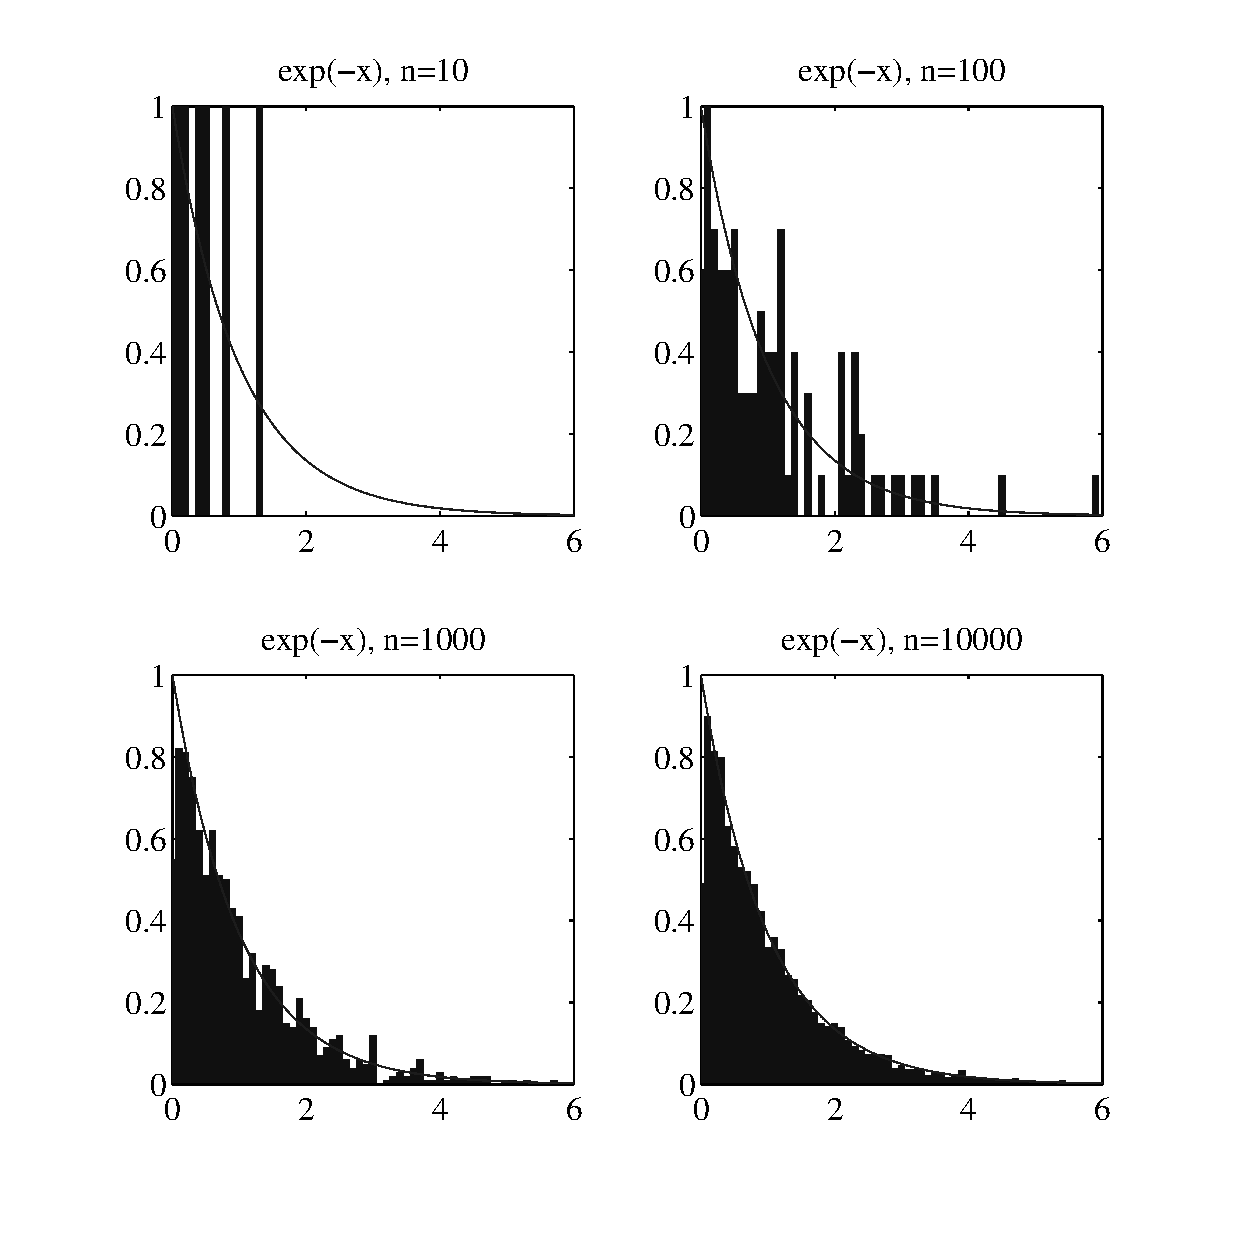
\includegraphics[width=\textwidth]{problem1}
\end{figure*}
\end{document}
